\clearpage
%//==============================--@--==============================//%
\subsection[4.3 Control Plane]{\hspace*{0.075 em}\raisebox{0.2 em}{$\pmb{\drsh}$} Control Plane}
\label{subsec:control-plane}

%//==============================--@--==============================//%
\subsubsection[4.3.1 Routing Protocols]{$\rightarrow$ Routing Protocols}
\label{subsubsec:routing-protocols}

%//==============================--@--==============================//%
\paragraph[4.3.1.1 Link-State Protocol]{$\pmb{\star}$ Link-State Protocol (centralized routing algorithm)}\mbox{}\\[4pt]
The link-state protocol discovers adjacency, broadcasts network topology, and implements Dijkstra's algorithm for the shortest paths. It involves:

\begin{itemize}
    \item \textbf{Adjacency discovery:} Routers exchange "hello" messages, discovering neighbors and establishing adjacencies (HELLO protocol).
    
    \item \textbf{Topology broadcast:} Routers create a \textbf{Link-State Advertisement (LSA)} containing adjacencies and broadcast it across the network.
    
    \item \textbf{Topology synchronization:} Routers maintain a \textbf{Link-State Database (LSDB)} storing LSAs, ensuring an identical and up-to-date network topology view.
    
    \item \textbf{Shortest path computation:} Routers use the LSDB and Dijkstra's algorithm to \underline{compute the shortest path tree, then populate forwarding tables} for destination-based forwarding.
\end{itemize}

\noindent Let us define the following notation:
\begin{itemize}[noitemsep, nolistsep]
    \item \texttt{D(v)}: cost of the least-cost path from the source node to destination \texttt{v} as of this
    iteration of the algorithm.
    \item \texttt{p(v)}: previous node (neighbor of \texttt{v}) along the current least-cost path from the
    source to \texttt{v}.
    \item \texttt{N'}: subset of nodes; \texttt{v} is in \texttt{N'} if the least-cost path from the source to \texttt{v} is definitively known.
\end{itemize}

\definecolor{codegray}{rgb}{0.5, 0.5, 0.5}
\definecolor{codeblack}{rgb}{0.0, 0.0, 1.0}
\definecolor{codeorange}{rgb}{0.8, 0.33, 0.0}
\definecolor{codered}{rgb}{1.0, 0.03, 0.0}
\begin{lstlisting}[language=, title={``Link-State (LS) Algorithm for Source Node \texttt{u}''\cite{Kurose2017}}, frame=tb, basicstyle=\scriptsize\ttfamily, escapechar=\%]
%\color{codeblack}initialization:%
    N' = {u}
    %\color{codeorange}for% all nodes v
        %\color{codeorange}if% v is a neighbor of u
            %\color{codeorange}then% D(v) = c(u,v)
        %\color{codeorange}else% D(v) = %$+\infty$%

%\color{codeblack}loop% {
    %\color{codeorange}find% w %\color{codered}not% in N' such that D(w) is a minimum
    %\color{codeorange}add% w to N'
    %\color{codeorange}update% D(v) %\color{codeorange}for% each neighbor v of w and %\color{codered}not% in N':
        D(v) = min(D(v), D(w)+ c(w,v))
    %\color{codegray}/* new cost to v is either old cost to v or known%
     %\color{codegray} * least path cost to w plus cost from w to v */%
} %\color{codeblack}until% N' = N
\end{lstlisting}

\vspace{1em}
\noindent \textbf{Pros \& Cons:}
\begin{table}[H]
    \begin{tabularx}{\linewidth}{>{\parskip1ex}X@{\kern4\tabcolsep}>{\parskip1ex}X}
    \toprule
    \hfil\bfseries Pros
    &
    \hfil\bfseries Cons 
    \\\cmidrule(r{3\tabcolsep}){1-1}\cmidrule(l{-\tabcolsep}){2-2}
    
    %% separated by empty line or \par
    Faster convergence, $\mathcal{O}(N^2)$, and more reliable path selection.\par
    Each router has a consistent view of the entire network topology.\par
    Resilient to routing loops.
    &
    
    %% separated by empty line or \par
    Higher memory and processing requi- rements.\par
    More complex and harder to trouble- shoot.\par
    May not scale well in very large networks.
    \\\bottomrule
    \end{tabularx}
    \caption{Pros \& cons: Link-State Protocol.}
\end{table}

\newpage
\noindent \textbf{Exemplo de execução do Link-State algorithm:}
\begin{figure}[H]
    \centering
    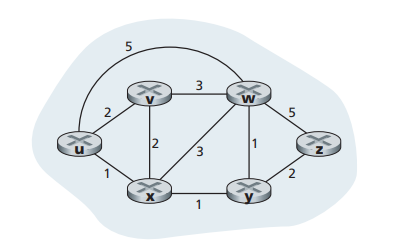
\includegraphics[width = 0.5\linewidth]{img/4/control-plane/state-link/graph-example.png}
    \caption{``Abstract graph model of a computer network''\cite{Kurose2017}}
    \label{fig:graph-example}
\end{figure}

\begin{figure}[H]
    \centering
    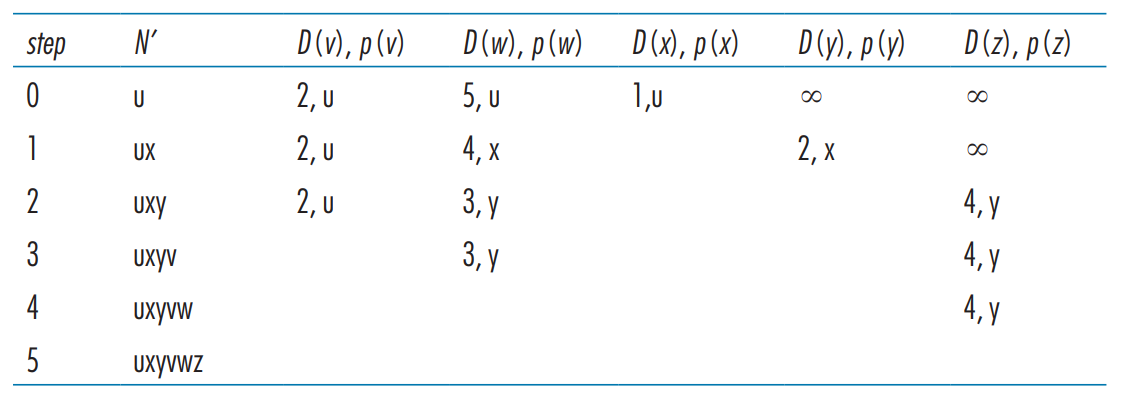
\includegraphics[width = 0.85\linewidth]{img/4/control-plane/state-link/dijkstra.png}
    \caption{``Running the link-state algorithm on the network''\cite{Kurose2017}}
    \label{fig:dijkstra}
\end{figure}

\begin{figure}[H]
    \centering
    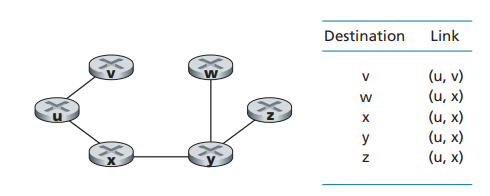
\includegraphics[width = 0.7\linewidth]{img/4/control-plane/state-link/shortest-path.png}
    \caption{``Least cost path and forwarding table for node \texttt{u}''\cite{Kurose2017}}
    \label{fig:shortest-path}
\end{figure}

%//==============================--@--==============================//%
\clearpage
\paragraph[4.3.1.2 Distance-Vector Protocols]{$\pmb{\star}$ Distance-Vector Protocols (decentralized routing algorithm)}\mbox{}

$$
    \text{\underline{Bellman-Ford equation:}} \quad \boxed{ D_\texttt{x}(\texttt{y}) = \min_\texttt{v}\{\, \text{c}(\texttt{x}, \texttt{v}) + D_\texttt{v}(\texttt{y})\, \} }
$$
Distance-vector protocols employ the Bellman-Ford algorithm to compute the shortest path. They involve:

\begin{itemize}
    \item \textbf{Routing table exchange:} Routers periodically exchange routing tables with neighbors, updating their tables accordingly.
    
    \item \textbf{Route selection:} Routers use the Bellman-Ford algorithm to update routing tables and determine the best path to each destination.
    
    \item \textbf{Count to infinity problem:} Slow convergence may lead to \underline{routing loops} and suboptimal paths. "Split horizon" and "poison reverse" techniques can mitigate this problem.
\end{itemize}

\definecolor{codegray}{rgb}{0.5, 0.5, 0.5}
\definecolor{codeblack}{rgb}{0.0, 0.0, 1.0}
\definecolor{codeorange}{rgb}{0.8, 0.33, 0.0}
\definecolor{codered}{rgb}{1.0, 0.03, 0.0}
\begin{lstlisting}[language=, title={``Distance-Vector (DV) Algorithm''\cite{Kurose2017}}, frame=tb, basicstyle=\scriptsize\ttfamily, escapechar=\%]
%\color{codeblack}initialization:%
    %\color{codeorange}for% all destinations y in N:
        %$\texttt{D}_\texttt{x}(\texttt{y})$% = c(x,y) %\color{codegray} /* if y is not a neighbor then c(x,y)= $+\infty$ */%
    %\color{codeorange}for% each neighbor w
        %$\texttt{D}_\texttt{w}(\texttt{y})$% = ? for all destinations y in N
    %\color{codeorange}for% each neighbor w
        %\color{codeorange}send% distance vector %$\texttt{D}_\texttt{x}$% = [%$\texttt{D}_\texttt{x}(\texttt{y})$%: y in N] to w

%\color{codeblack}loop% {
    %\color{codered}wait% %\color{codeorange}until% 
        I see a link cost change to some neighbor w
    %\color{codeorange}or until% 
        I receive a distance vector from some neighbor w
    
    %\color{codeorange}for% each y in N:
        %$\texttt{D}_\texttt{x}(\texttt{y})$% = min_v{c(x,v) + %$\texttt{D}_\texttt{v}(\texttt{y})$%}
    
    %\color{codeorange}if% %$\texttt{D}_\texttt{x}(\texttt{y})$% changed for any destination y
        %\color{codeorange}send% distance vector %$\texttt{D}_\texttt{x}$% = [%$\texttt{D}_\texttt{x}(\texttt{y})$%: y in N] to all neighbors
} %\color{codeblack}forever%
\end{lstlisting}

\vspace{1em}
\noindent \textbf{Addressing Routing Loops in Distance-Vector Protocols:}
\begin{itemize}
    \item \textbf{Routing loops} occur when a packet is forwarded in a continuous loop between routers, causing degraded network performance and packet loss. They often result from incorrect routing information due to slow convergence or the count-to-infinity issue in distance-vector protocols.

    \item The \textbf{count-to-infinity} issue arises when routers incrementally update their routing tables with outdated information, causing the routing metric to increase indefinitely. This can lead to suboptimal routing decisions and loops.
    
    \item \textbf{Split horizon} prevents routing loops by not propagating routing information learned from a neighbor back to that same neighbor, avoiding the spread of incorrect routing information.
    
    \item \textbf{Poison reverse} mitigates routing loops by advertising unreachable destinations with an infinite metric, informing neighbors not to use the advertising router as a path to the destination.
    
    \item Combining \textbf{split horizon} and \textbf{poison reverse} techniques can effectively prevent and resolve routing loops, leading to a more stable and efficient network.
\end{itemize}

\newpage
\noindent \textbf{Pros \& Cons:}
\begin{table}[H]
    \begin{tabularx}{\linewidth}{>{\parskip1ex}X@{\kern4\tabcolsep}>{\parskip1ex}X}
    \toprule
    \hfil\bfseries Pros
    &
    \hfil\bfseries Cons 
    \\\cmidrule(r{3\tabcolsep}){1-1}\cmidrule(l{-\tabcolsep}){2-2}
    
    %% separated by empty line or \par
    Lower computational requirements com- pared to link-state protocols.\par
    Simpler to configure and maintain.
    &
    
    %% separated by empty line or \par
    Slower convergence, $\mathcal{O}(N \cdot E)$, leading to temporary routing loops and suboptimal paths.\par
    Limited network visibility.\par
    May not scale well in large networks due to the periodic exchange of routing tables.
    \\\bottomrule
    \end{tabularx}
    \caption{Pros \& cons: Distance-Vector Protocols.}
\end{table}

\noindent \textbf{Exemplo de execução do Distance-Vector algorithm:}
\begin{figure}[H]
    \centering
    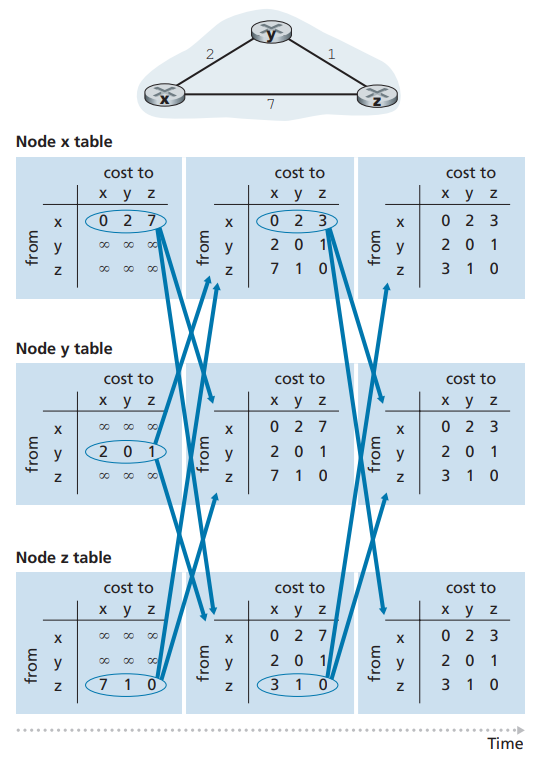
\includegraphics[width = 0.75\linewidth]{img/4/control-plane/distance-vector/DV-example.png}
    \caption{``Distance-vector (DV) algorithm in operation''\cite{Kurose2017}}
    \label{fig:shortest-path-DV}
\end{figure}

%//==============================--@--==============================//%
\clearpage
\paragraph[4.3.1.3 Path-Vector Protocols]{$\pmb{\star}$ Path-Vector Protocols}\mbox{}\\[4pt]
Path-vector routing protocols extend distance-vector protocols by sharing the entire path information to a destination. They involve:

\begin{itemize}
    \item \textbf{Path advertisement:} Routers advertise the entire path to each destination, instead of just the distance.
    
    \item \textbf{Path selection:} Routers use advertised paths to select the best path to each destination based on criteria such as path length, reliability, or administrative preferences.
    
    \item \textbf{Preventing routing loops:} Routers detect and prevent routing loops by checking for their own presence in the advertised path.
\end{itemize}

\vspace{1em}
\noindent \textbf{Pros \& Cons:}
\begin{table}[H]
    \begin{tabularx}{\linewidth}{>{\parskip1ex}X@{\kern4\tabcolsep}>{\parskip1ex}X}
    \toprule
    \hfil\bfseries Pros
    &
    \hfil\bfseries Cons 
    \\\cmidrule(r{3\tabcolsep}){1-1}\cmidrule(l{-\tabcolsep}){2-2}
    
    %% separated by empty line or \par
    More accurate and reliable path selection compared to distance-vector protocols.\par
    Prevents routing loops by detecting and discarding paths containing the router's own ID.\par
    Supports policy-based routing by allowing administrators to define routing preferences.
    &
    
    %% separated by empty line or \par
    Path advertisement can increase message size and bandwidth consumption.\par
    Requires more memory and processing power than distance-vector protocols, but less than link-state protocols.\par
    Less straightforward than distance-vector protocols in terms of configuration and troubleshooting.
    \\\bottomrule
    \end{tabularx}
    \caption{Pros \& cons: Path-Vector Protocols.}
\end{table}

%//==============================--@--==============================//%
\subsubsection[4.3.2 Hierarchical Routing and Autonomous Systems]{$\rightarrow$ Hierarchical Routing and Autonomous Systems}
\label{subsec:hierarchical-routing-autonomous-systems}

Hierarchical routing simplifies large-scale network routing by organizing the topology into hierarchical levels, reducing routing information, and improving scalability and convergence times.

\begin{itemize}
    \item \textbf{Autonomous Systems (ASes):} Collections of IP networks and routers controlled by a single organization with a common routing policy. The Internet is divided into thousands of ASes, each with a unique AS number.
    
    \item \textbf{Levels:} Hierarchical routing divides networks into tiers, such as core and edge, or additional levels like regional or local tiers.
    
    \item \textbf{Addressing:} Each hierarchy level has a unique address space, enabling efficient address aggregation and route summarization.
    
    \item \textbf{Route Aggregation and Summarization:} Higher-level routers maintain summarized routes, reducing the number of routes to store and exchange, and conserving resources.
    
    \item \textbf{Isolation:} Hierarchical routing isolates failures and updates within specific hierarchy levels or ASes, preventing network-wide instability.
\end{itemize}

\noindent Hierarchical routing is employed in both intradomain and interdomain routing, with OSPF and BGP using area or AS hierarchies. Intradomain routing within an AS uses protocols like OSPF, while interdomain routing between ASes is achieved through BGP.

%//==============================--@--==============================//%
\subsubsection[4.3.2 Intra-AS Routing in the Internet]{$\rightarrow$ Intra-AS Routing in the Internet}
\label{subsubsec:AS-protocols}

%//==============================--@--==============================//%
\paragraph[4.3.2.1 RIP: Routing Information Protocol]{$\pmb{\star}$ RIP: Routing Information Protocol}\mbox{}\\[4pt]
RIP is a distance-vector routing protocol that uses hop count as the metric for selecting the best path. It has a maximum hop count limit of 15, which restricts its scalability. Operates on top of UDP.

\begin{itemize}
    \item \textbf{RIP Inner Workings}: RIP routers exchange their routing tables every 30 seconds. Upon receiving an update, a router will compare the received routes with its own routing table and update its entries if a shorter path is found.
\end{itemize}

%//==============================--@--==============================//%
\paragraph[4.3.2.2 OSPF: Open Shortest Path First]{$\pmb{\star}$ OSPF: Open Shortest Path First}\mbox{}\\[4pt]
OSPF is a link-state routing protocol that calculates the shortest path using Dijkstra's algorithm. It is hierarchical and supports areas, allowing for better scalability compared to RIP.

\begin{itemize}
    \item OSPF is a widely used, open, link-state routing protocol for intra-AS routing.
    \item Routers construct a complete topological map of the AS and use Dijkstra's algorithm to determine shortest-path trees.
    \item Link costs can be configured by the network administrator, OSPF does not dictate how they are set.
    \item Routers broadcast routing information to all routers in the AS, not just their neighbors.
    \item Link-state information is broadcasted when a link's state changes or at least once every 30 minutes for robustness.
    \item \underline{OSPF messages are carried by IP} with an upper-layer protocol number of 89.
    \item The OSPF protocol implements functionality for reliable message transfer, link-state broadcast, link health check, and database synchronization with neighbors.
\end{itemize}

\noindent OSPF provides:

\begin{itemize}
    \item \textbf{Security:} OSPF supports authentication (simple and MD5) to prevent unauthorized routers from injecting incorrect information.
    \item \textbf{Multiple same-cost paths:} OSPF allows load balancing over multiple equal-cost paths.
    \item \textbf{Integrated support for unicast and multicast routing:} Multicast OSPF (MOSPF) extends OSPF to support multicast routing.
    \item \textbf{Support for hierarchy within a single AS:}
    \begin{itemize}[noitemsep, nolistsep]
        \item OSPF AS can be divided into areas, each running its own link-state routing algorithm.
        \item Area border routers handle routing between areas.
        \item One OSPF area is designated as the backbone area, which routes traffic between other areas.
    \end{itemize}
\end{itemize}

%//==============================--@--==============================//%
\clearpage
\subsubsection[4.3.3 Inter-AS Routing in the Internet]{$\rightarrow$ Inter-AS Routing in the Internet}
\label{subsubsec:inter-as}

%//==============================--@--==============================//%
\paragraph[4.3.3.1 BGP: Border Gateway Protocol]{$\pmb{\star}$ BGP: Border Gateway Protocol}\mbox{}\\[4pt]
BGP is a path-vector routing protocol designed for inter-domain routing between Autonomous Systems (ASes). It is crucial for the global Internet routing infrastructure.

\vspace{1 em}
\noindent BGP provides each router a means to:
\begin{itemize}
    \item Obtain prefix reachability information from neighboring ASes (allows each subnet to advertise its existence).
    \item Determine the “best” routes to the prefixes.
\end{itemize}

\noindent\textbf{Advertising BGP Route Information:} BGP routers, also known as "peers" or "neighbors," exchange routing updates containing the entire AS-path information. BGP uses various attributes, such as AS-path length and local preference, to select the best path.

\begin{itemize}
    \item \textbf{eBGP:} External BGP is used to exchange routing information between ASes.
    \item \textbf{iBGP:} Internal BGP is used to exchange routing information within the same AS.
\end{itemize}

\vspace{-1.0 em}
\begin{figure}[H]
    \centering
    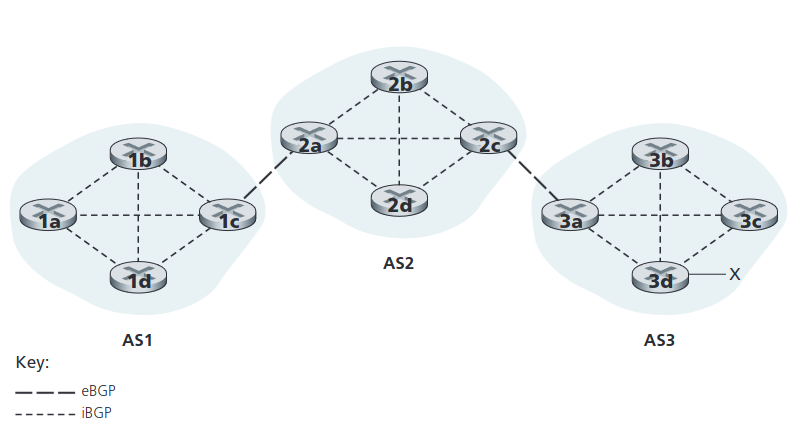
\includegraphics[width = 0.825\linewidth]{img/4/control-plane/BGP/BGP.png}
    \caption{eBGP and iBGP connections. Notice that iBGP connections do not necessarily follow the physical link between routers, in order to propagate the reachability information, both iBGP and eBGP sessions are used.}
    \label{fig:BGP}
\end{figure}

\renewcommand*{\thefootnote}{\fnsymbol{footnote}}
\footnotetext[4]{%
    \noindent\textbf{Commercial Routing Between Autonomous Systems} \mbox{}
    
    \noindent In the context of commercial routing, ASes can establish various types of relationships, such as transit, peering, or customer-provider relationships. These relationships dictate how routing information is exchanged and propagated through the Internet.
    
    \begin{itemize}
        \item \textbf{Transit:} A transit AS provides connectivity for other ASes to reach the global Internet. Transit providers typically charge for their services.
        
        \item \textbf{Peering:} In a peering relationship, two ASes agree to exchange routing information without charging each other. This is commonly established between ISPs of similar size for mutual benefit.
        
        \item \textbf{Customer-Provider:} In this relationship, a provider AS offers Internet access and routing services to a customer AS. The customer typically pays the provider for the services.
    \end{itemize}
}
\renewcommand*{\thefootnote}{\arabic{footnote}}

\newpage
\noindent\textbf{Route Selection in BGP}\mbox{}

\noindent Determining the Best Routes in BGP involves considering multiple paths from a given router to a destination subnet. BGP routers often receive reachability information about dozens of different possible paths. A router chooses among these paths and configures its forwarding table accordingly. When a router advertises a prefix across a BGP connection, it includes several BGP attributes, such as \texttt{AS-PATH} and \texttt{NEXT-HOP}, with the prefix.

\begin{itemize}
    \item \textbf{AS-PATH} contains the list of ASes traversed by the advertisement. Routers use the \texttt{AS-PATH} attribute to detect and prevent looping advertisements by rejecting advertisements containing their own AS in the path list. 

    \item \textbf{NEXT-HOP} is the IP address of the router interface that begins the \texttt{AS-PATH}. It serves as the critical link between inter-AS and intra-AS routing protocols.

    \item \textbf{LOCAL-PREF} is a BGP attribute representing the local preference value assigned to a route within an AS. This value is not passed outside the AS and is used to select the preferred exit point from the AS for a given route. The higher the local preference value, the more preferred the route.

    \item \textbf{MED} (Multi-Exit Discriminator) is another BGP attribute used to influence the choice of entry point to an AS for incoming traffic. The \texttt{MED} value suggests the preferred entry point by comparing the \texttt{MED} values of different routes advertised by neighboring ASes. The lower the \texttt{MED} value, the more preferred the route.
\end{itemize}

\begin{figure}[H]
    \centering
    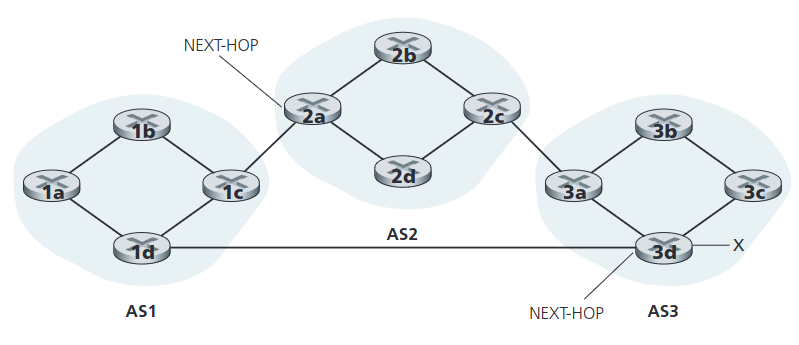
\includegraphics[width = 0.825\linewidth]{img/4/control-plane/BGP/route.png}
    \caption{The IP address of the leftmost interface of router 3d and of router 2a are known as Next-Hop.}
    \label{fig:route}
\end{figure}

\noindent\textbf{Hot Potato Routing Algorithm}\mbox{}

\noindent Hot potato routing, also known as "early-exit" or "closest-exit" routing, is a strategy used to select the best path based on the shortest internal distance within an AS. Hot potato is a selfish algorithm: it tries to reduce the cost in its own AS while ignoring the other components of the end-to-end costs outside its AS.

\begin{figure}[H]
    \centering
    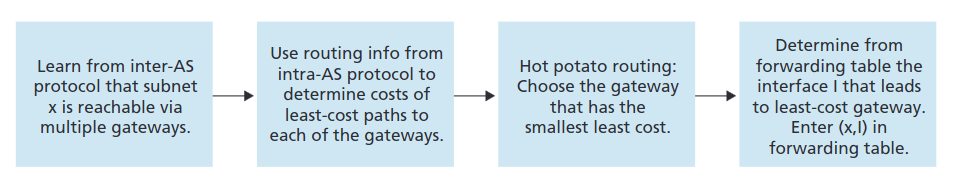
\includegraphics[width = 0.85\linewidth]{img/4/control-plane/BGP/hot-potato.png}
    \caption{Hot potato algorithm \cite{Kurose2017}}
    \label{fig:Hot-potato}
\end{figure}

\noindent\textbf{BGP Route-Selection Algorithm}\mbox{}

\noindent In practice, BGP uses a more sophisticated route-selection algorithm that incorporates Hot Potato Routing and takes \texttt{LOCAL-PREF} and \texttt{MED} into account. For any given destination prefix, the input into BGP's route-selection algorithm is the set of all routes to that prefix that have been learned and accepted by the router. BGP sequentially invokes the following elimination rules until one route remains:

\begin{enumerate}
    \item Select the routes with the highest local preference values (\texttt{LOCAL-PREF}).
    \item From the remaining routes, select the route with the shortest \texttt{AS-PATH}.
    \item From the remaining routes, choose the route with the lowest \texttt{MED} value.
    \item From the remaining routes, use Hot Potato Routing to select the route with the closest \texttt{NEXT-HOP} router.
    \item If more than one route still remains, use other BGP identifiers to select the route.
\end{enumerate}

\noindent\textbf{Route Filtering and Policy Control in BGP}\mbox{}

\noindent BGP provides various methods for filtering and controlling route advertisements to implement routing policies.

\begin{itemize}
    \item \textbf{Prefix Lists:} Used to filter routes based on the IP prefix.
    
    \item \textbf{AS-PATH Access Lists:} Used to filter routes based on the \texttt{AS-PATH} attribute.
    
    \item \textbf{Route Maps:} Used to apply complex policies that involve multiple BGP attributes. Route maps can manipulate attributes or filter routes based on various criteria.

    \item Each AS may choose to \underline{not} advertise their routes to neighbouring ASes.

    \item Each AS attributes a preference value to the routes advertised by their neighbors.
\end{itemize}

\noindent By utilizing these filtering and policy control methods, BGP allows network administrators to manage inter-domain routing and implement policies based on commercial agreements or traffic engineering requirements.

\begin{itemize}
    \item \textbf{AS routing policy can trump other considerations}, such as shortest AS path or hot potato routing; local-preference attribute value is fixed by the policy of the local AS.
    
    \item \underline{Access ISP\footnotemark[4] networks (last-mile/local ISPs)} \textbf{advertise no paths to any other destinations except themselves}, ensuring all traffic leaving/entering them must have the source/destination within their own network.

    \item The rule of thumb followed by commercial ISPs: \textbf{any traffic flowing across an ISP's backbone network must have either a source or a destination (or both) in a network that is a \underline{customer of that ISP}}.
    
    \item Differences between inter-AS and intra-AS routing protocols: Policy (dominates in inter-AS routing), Scale (critical for inter-AS routing, less so for intra-AS routing), and Performance (less important in inter-AS routing due to policy constraints).
\end{itemize}

\footnotetext[4]{%
    Access ISPs are usually connected to higher-tier ISPs, such as Tier-1 or Tier-2 ISPs, which have broader network coverage and provide backbone connectivity for lower-tier ISPs. In this sense, access ISPs are at the bottom of the ISP hierarchy, as they primarily focus on providing Internet services directly to the end-users.
}

%//==============================--@--==============================//%
